\documentclass[12pt]{article}
\usepackage{algpseudocode}
\usepackage{graphicx}
\usepackage{subfiles}
\usepackage{svg}
\usepackage{pdfpages}
\usepackage{hyperref}
\hypersetup{
    bookmarks=true,         % show bookmarks bar?
    unicode=false,          % non-Latin characters in Acrobat’s bookmarks
    pdftoolbar=true,        % show Acrobat’s toolbar?
    pdfmenubar=true,        % show Acrobat’s menu?
    pdffitwindow=false,     % window fit to page when opened
    pdfstartview={FitH},    % fits the width of the page to the window
    pdftitle={COMP9900 Capstone Project Proposal, Investment Simulator},    % title
    pdfauthor={Jihad Maraachli, Khan Schroder-Turner, Kovid Sharma, Simon Garrod, Timothy Brunette
},     % author
    pdfsubject={},   % subject of the document
    pdfcreator={},   % creator of the document
    pdfproducer={}, % producer of the document
    pdfkeywords={software, web development, investing, investment simulator}, % list of keywords
    pdfnewwindow=true,      % links in new PDF window
    colorlinks=false,       % false: boxed links; true: colored links
    linkcolor=red,          % color of internal links (change box color with linkbordercolor)
    citecolor=green,        % color of links to bibliography
    filecolor=cyan,         % color of file links
    urlcolor=        % color of external links
}


\usepackage{listings}
\usepackage{setspace}
\onehalfspacing
\usepackage{appendix}
\usepackage[margin=2.5cm]{geometry}
\usepackage[ruled,linesnumbered, noend, vlined]{algorithm2e}
\usepackage{amsmath,amsthm,amssymb}
\usepackage{parskip}
\usepackage{url}
\usepackage{authblk}
\setlength{\parindent}{0mm}

\usepackage{titlesec}
\usepackage{mathtools}
\usepackage{amstext}
\usepackage{stackengine}
\usepackage{chngcntr}
\usepackage{adjustbox}
\usepackage{etoolbox}
\usepackage{booktabs, multicol, multirow}
\usepackage{subcaption}
\usepackage[nottoc,numbib]{tocbibind}
\usepackage{enumitem}
\usepackage{gensymb}
\usepackage{pdflscape}

\usepackage{array}   % for \newcolumntype macro

\counterwithin*{equation}{section}
\counterwithin*{equation}{subsection}

\newcommand{\sectionbreak}{\clearpage}
\newlength{\textundbildtextheight}

\algdef{SE}[SUBALG]{Indent}{EndIndent}{}{\algorithmicend\ }%
\algtext*{Indent}
\algtext*{EndIndent}

\usepackage[backend=biber]{biblatex}
\usepackage{csquotes}

\bibliographystyle{apalike}
\bibliography{bibliography.bib}% Syntax for version >= 1.2



\title{COMP9900 Capstone Project Proposal\\

\large Investment Simulator
}


\author{
  Jihad Maraachli\\
  \small z5156156\\
  \href{mailto:j.meraachli@student.unsw.edu.au}{j.meraachli@student.unsw.edu.au}
  \and
  Khan Schroder-Turner\\
  \small z5020362\\
  \href{mailto:k.schroder-turner@student.unsw.edu.au}{k.schroder-turner@student.unsw.edu.au}
  \and
  Kovid Sharma\\
  \small z5240067\\
  \href{mailto:k.sharma.1@student.unsw.edu.au}{k.sharma.1@student.unsw.edu.au}
  \and
  Simon Garrod\\
  \small z3264122\\
  \href{mailto:simon@unsw.edu.au}{simon@unsw.edu.au}
  \and
  Timothy Brunette\\
  \small z5233368\\
  \href{mailto:t.brunette@student.unsw.edu.au}{t.brunette@student.unsw.edu.au}
}



\begin{document}
    \maketitle
    \newpage



    \tableofcontents
    \thispagestyle{empty}

    % !TEX root = ..\proposal.tex

\section{Introduction}
    \label{sec:intro}



People often seek investment vehicles as a method to expand their savings, diversify their savings portfolio and grow their wealth. Several investment vehicles are available for investors to achieve the goals of diversification and value creation such as bonds, stocks, options, and derivatives. Each of these requires extensive skills and domain knowledge to master. Given the focus on stock market within the spectrum of this project, our aim is to advance the skill sets of our users to ensure that stock trading risks are properly acknowledged and appreciated. 

Traditionally, stock trading and investing in public companies was considered exclusive to high-value portfolios. Such accounts historically had a dedicated broker who communicated the buying and selling of stocks (orders) over the phone. With the advancement of technology, exchange mediums have become readily available from the convenience of a person's computer, tablet, or even smartphone. Technological advancement has opened the doors for many new investors and traders to enter the world of stock investing, though they are often lured in by marketing campaigns for particular products and `get rich quick’ schemes. The stock market can be an endless maze for new traders who are often lost in the labyrinth of technical terms and financial lingo. Additionally, high frequency trading has put the retail traders/trading at a disadvantage against huge machines and servers which trade at the microsecond-level using advanced analysis based on market changes, data releases, and news sentiment. This creates yet another barrier for the retail traders who are already hesitant so they might miss the chance of learning about the stock market or, on the other end of the spectrum, are under the impression that the stock market is a money making machine, resulting in uninformed and high risk investments.

To combat the aforementioned hurdles that retail traders often faced, we aim to create a virtual market ecosystem allowing traders and investors access to a unique experience that mimics the real stock exchange medium with virtual money. The user is given a set amount of virtual money to simu-buy or simu-sell shares (and potentially cryptocurrency) in order to test the investment strategy rather than risking the user’s own capital. The virtual market allows the users to evaluate the decisions taken in the short and long term by measuring portfolio yield in terms of absolute return and relative return. Our platform will allow traders to avoid falling into the marketing gimmicks and false advertisements by enabling them to test an investment strategy before real capital is at risk. This lets our users make better and more informed decisions about their chosen strategy, allowing them to accurately judge whether they need more knowledge or training prior to investing their hard-earned money into the stock market.

    % !TEX root = ..\proposal.tex


\section{Background}
    \label{sec:background}

\subsection{Problem Statement}
    \label{subsec:problem_statement}
    
Although many systems exist that tackle the virtualisation of a trading ecosystem, many fall short of the intended goal; to create a real experience for the users to better understand the risks involved in trading the stock market and to asses their skill sets. Such systems are often linked to real cash trading brokers who wish to capitalise on the virtual ecosystem offering. This is done through making the virtual account available for only a limited amount of time (e.g. 1 week or 1 month) before the account is automatically closed. After this, these systems often try to lure the user into depositing real money and start real trading. A short duration of time is not sufficient to tackle a full experience within the stock market given its long-term nature as opposed to other trading instruments such as Forex trading and options trading. Our systems aims to fill the gap through offering an open-ended virtual accounts with no termination date in order to ensure that our users can benefit from an effective marketplace to learn, observe, and trade virtual stocks rather than learning through blowing up their own accounts and potentially losing their real money.

\subsection{Existing Systems}
\label{subsec:existing_systems}
    
There are several systems that offer similar services; 
\begin{enumerate}
    \item \href{https://www.investopedia.com/simulator/portfolio/nogamestotradein.aspx}{Investopedia Stock Simulator}\label{alt:investop}
    \item \href{https://app.wallstreetsurvivor.com/}{Wall Street Survivor} \label{alt:wallst}
    \item \href{https://www.stocktrak.com/}{Stock Trak}\label{alt:stocktrak}
    \item \href{https://www.howthemarketworks.com/}{HOWTHEMARKETWORKS}\label{alt:howmarket}
    \item \href{https://www.asx.com.au/education/sharemarket-game.htm}{Sharemarket Game}\label{alt:sharegame}
\end{enumerate}

Each alternative has a varying feature set, notably item \ref{alt:howmarket} is the most well developed of the options. It has all of the base features required in the project brief, and many additional features. The interface is markedly the best of the alternatives, though doesn't come without some features to be desired, these are described in Table \ref{tab:drawbacks} below.
    
The poorest of the options is item \ref{alt:investop}, having limited functionality and a poor interface resulting in an unpleasant user experience. The website doesn't re-size correctly, provide announcements or a news feed for watched or bought investments or have a watch list feature. This is quickly followed by item \ref{alt:sharegame}; though it has more features, the interface is similarly awkward and limits users to Australian companies.
    
All options except for item \ref{alt:stocktrak} are free. Hence, it was not possible to evaluate the disadvantages of the platform outside of the disadvantage that it is not a free service. This disadvantage alone is a large deterrent for many users when there are other high quality platforms available.
    
A common draw back among all the alternatives is the UX design and interface. The designs across all platforms are either aesthetically unpleasing, or mirror standard enterprise designs for charting and usability. The interfaces are either unpleasant or un-intuitive, with the exception of item \ref{alt:howmarket} which is simply too cluttered although being straight forward; and even it has mismatched design themes throughout the site.
    

\begin{table}[htbp]
  \centering
  \caption{Alternative Drawbacks}\label{tab:drawbacks}
    \begin{tabular}{r|p{20.285em}}
    \textbf{Alternative} & \multicolumn{1}{l}{\textbf{Drawbacks}} \\
    \midrule
    Investopedia Stock Simulator (Item \ref{alt:investop}) & Poor interface\newline{}Have to join a competition to use the platform\newline{}No watchlist \newline{}No excel or CSV export of portfolio or trade history \\
    \midrule
    Wall Street Survivor (Item \ref{alt:wallst}) & Clunky interface, hard to navigate, inconsistent theming\newline{}No option for percentage fee when making trades\newline{}Trading search is buggy\newline{}No excel or CSV export of portfolio or trade history \\
    \midrule
    Stock Trak (Item \ref{alt:stocktrak}) & Paid service (as such other features cannot be compared) \\
    \midrule
    HOWTHEMARKETWORKS (Item \ref{alt:howmarket}) & Limited timescales for portfolio viewer\newline{}Best interface of the alternatives, but very cluttered and noisy in parts of the application \newline{} Inconsistent design themes in places\newline{}Can only compare to one indices at a time\newline{}Can't compare multiple user portfolios \\
    \midrule
    Sharemarket Game (Item \ref{alt:sharegame})& Can only participate in stock games, no running performance\newline{}Clunky and confusing interface, particularly for buying/selling - have to select company from drop down\newline{}Buggy graphs and dashboard \newline{}Only ASX shares \newline{}No excel or CSV export of portfolio\\
    \end{tabular}%
  \label{tab:addlabel}%
\end{table}%




% Possible differentiator - scenario modeller, prize pool (\$1 - \$5 entry fee, split up pool; amongst top 3, top 10 get entry fee back/ or free entry into next comp), recommended stocks, multiple portfolios, compare to interest rate from bank/term deposit/bonds/property (i.e. a benchmark), mixed portfolio models
    % !TEX root = ..\proposal.tex

\section{User Stories}
    \label{sec:user_stories}

    % !TEX root = ..\proposal.tex

\section{Story Boards}
    \label{sec:story_boards}

This section presents the story boards to outline the basic functionalities of the investment simulator. Storyboarding helps develop a sense of how the system will look, and how users can interact with it before it is formally designed and developed. 

The design of the wireframes and the story boards, are driven by two main usability principles: aesthetics/minimalist design and efficiency. We intend to develop a system that enables the investor to search for investment opportunities in an accessible and clutter-free environment. Additionally, the design incorporates efficiency in every aspect where buy investors can access their portfolio, execute transactions, and watch stocks with a few clicks. It should be noted that these storyboards are not to be taken for complete, concrete designs, as they are only used here to illustrate the users flow and interaction with the system.

\subsection{User Login}
\begin{figure}[h]
    \centering
    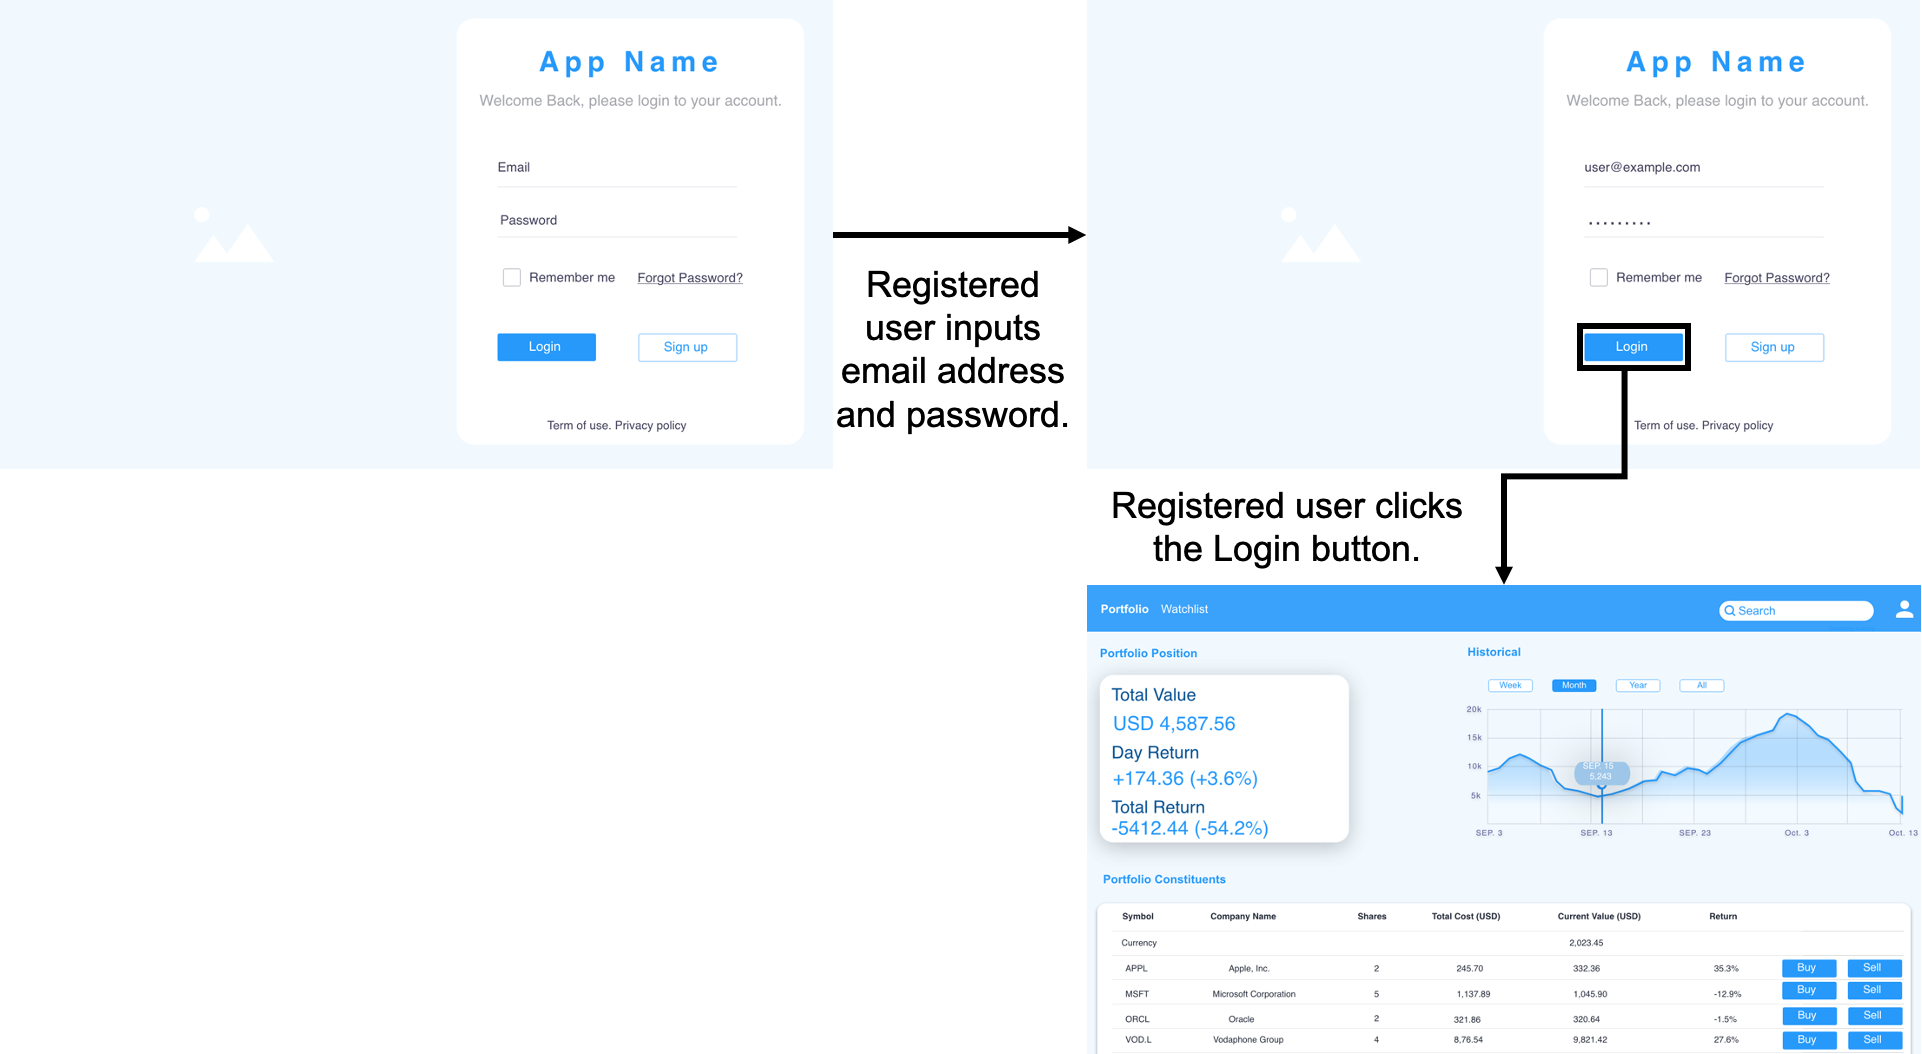
\includegraphics[scale = 0.5]{./3_story_boards/Login.png}
    \caption{Login wire-frame}
    \label{fig:login}
\end{figure}
\break


\subsection{User Sign-up}
\begin{figure}[h]
    \centering
    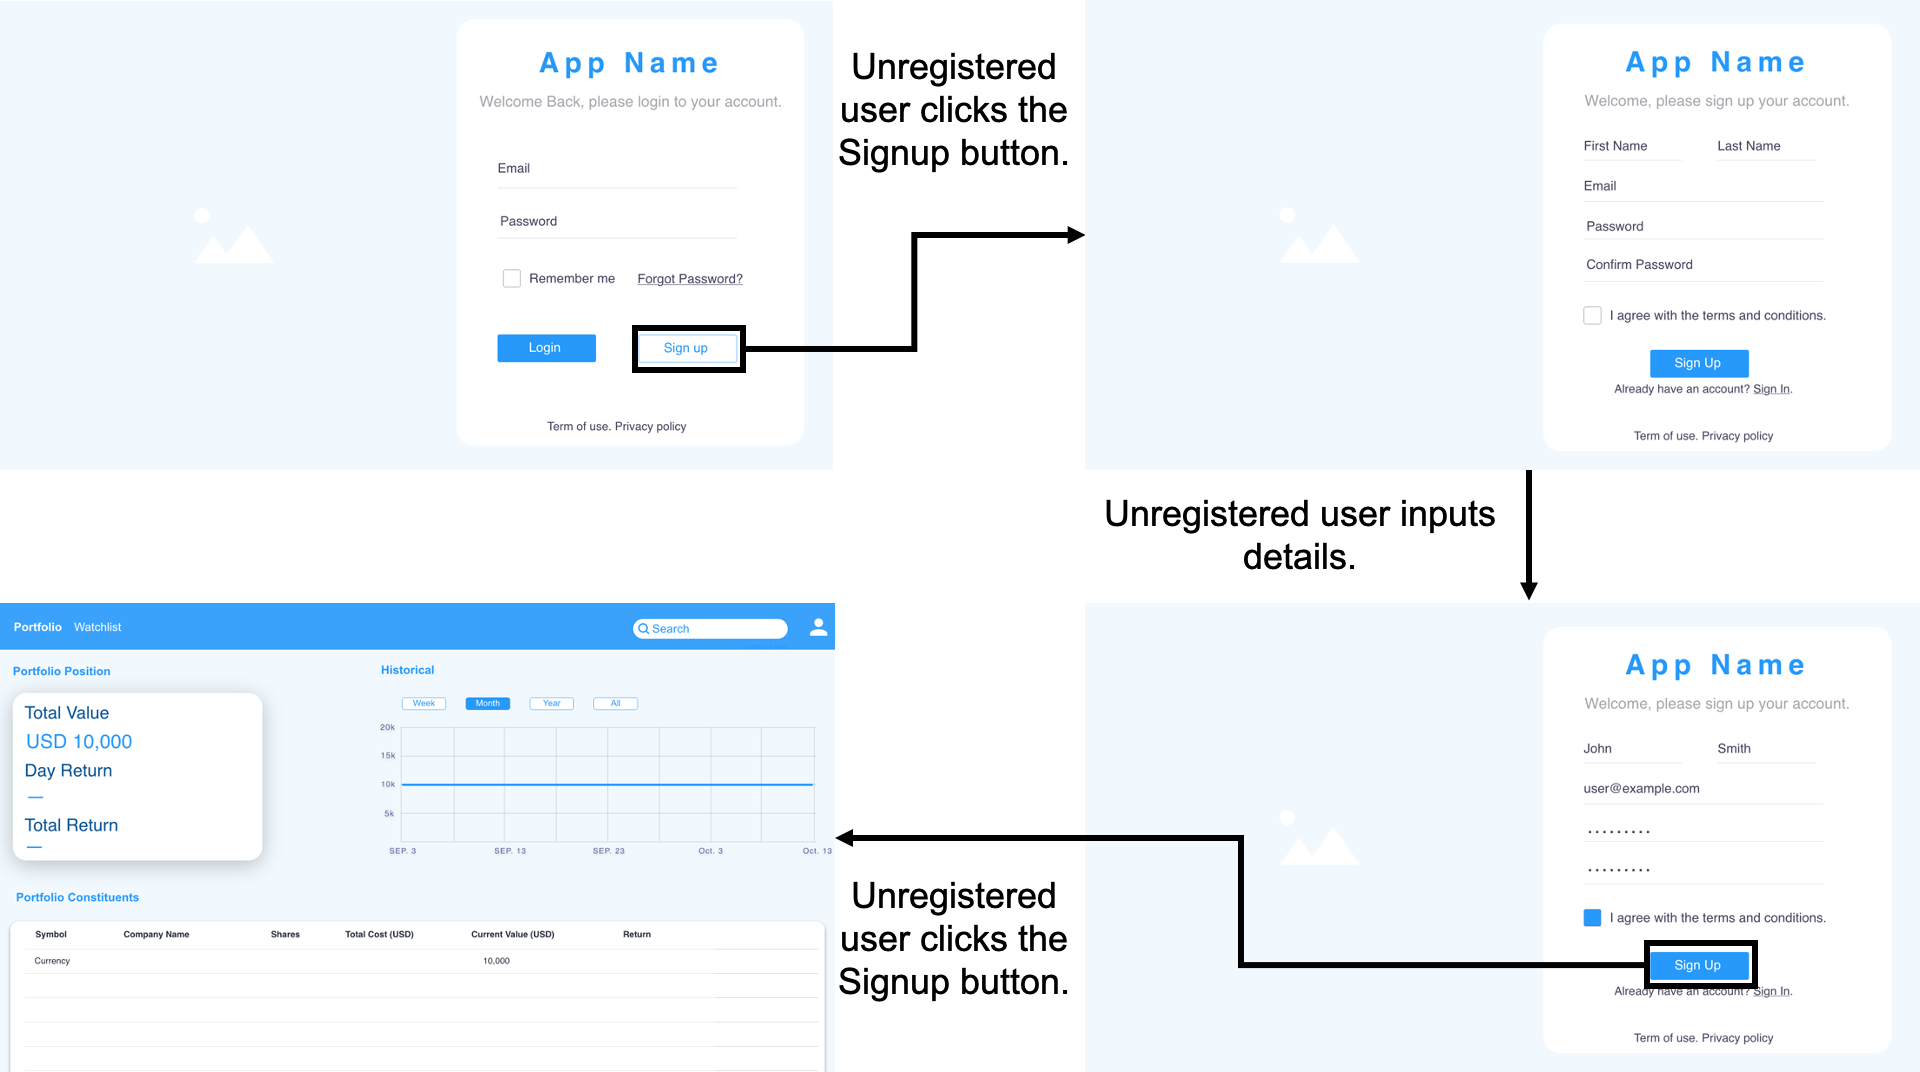
\includegraphics[scale = 0.5]{./3_story_boards/Signup.png}
    \caption{Sign-up wire-frame}
    \label{fig:signup}
\end{figure}
\break


\subsection{Search and Watchlist}
\begin{figure}[h]
    \centering
    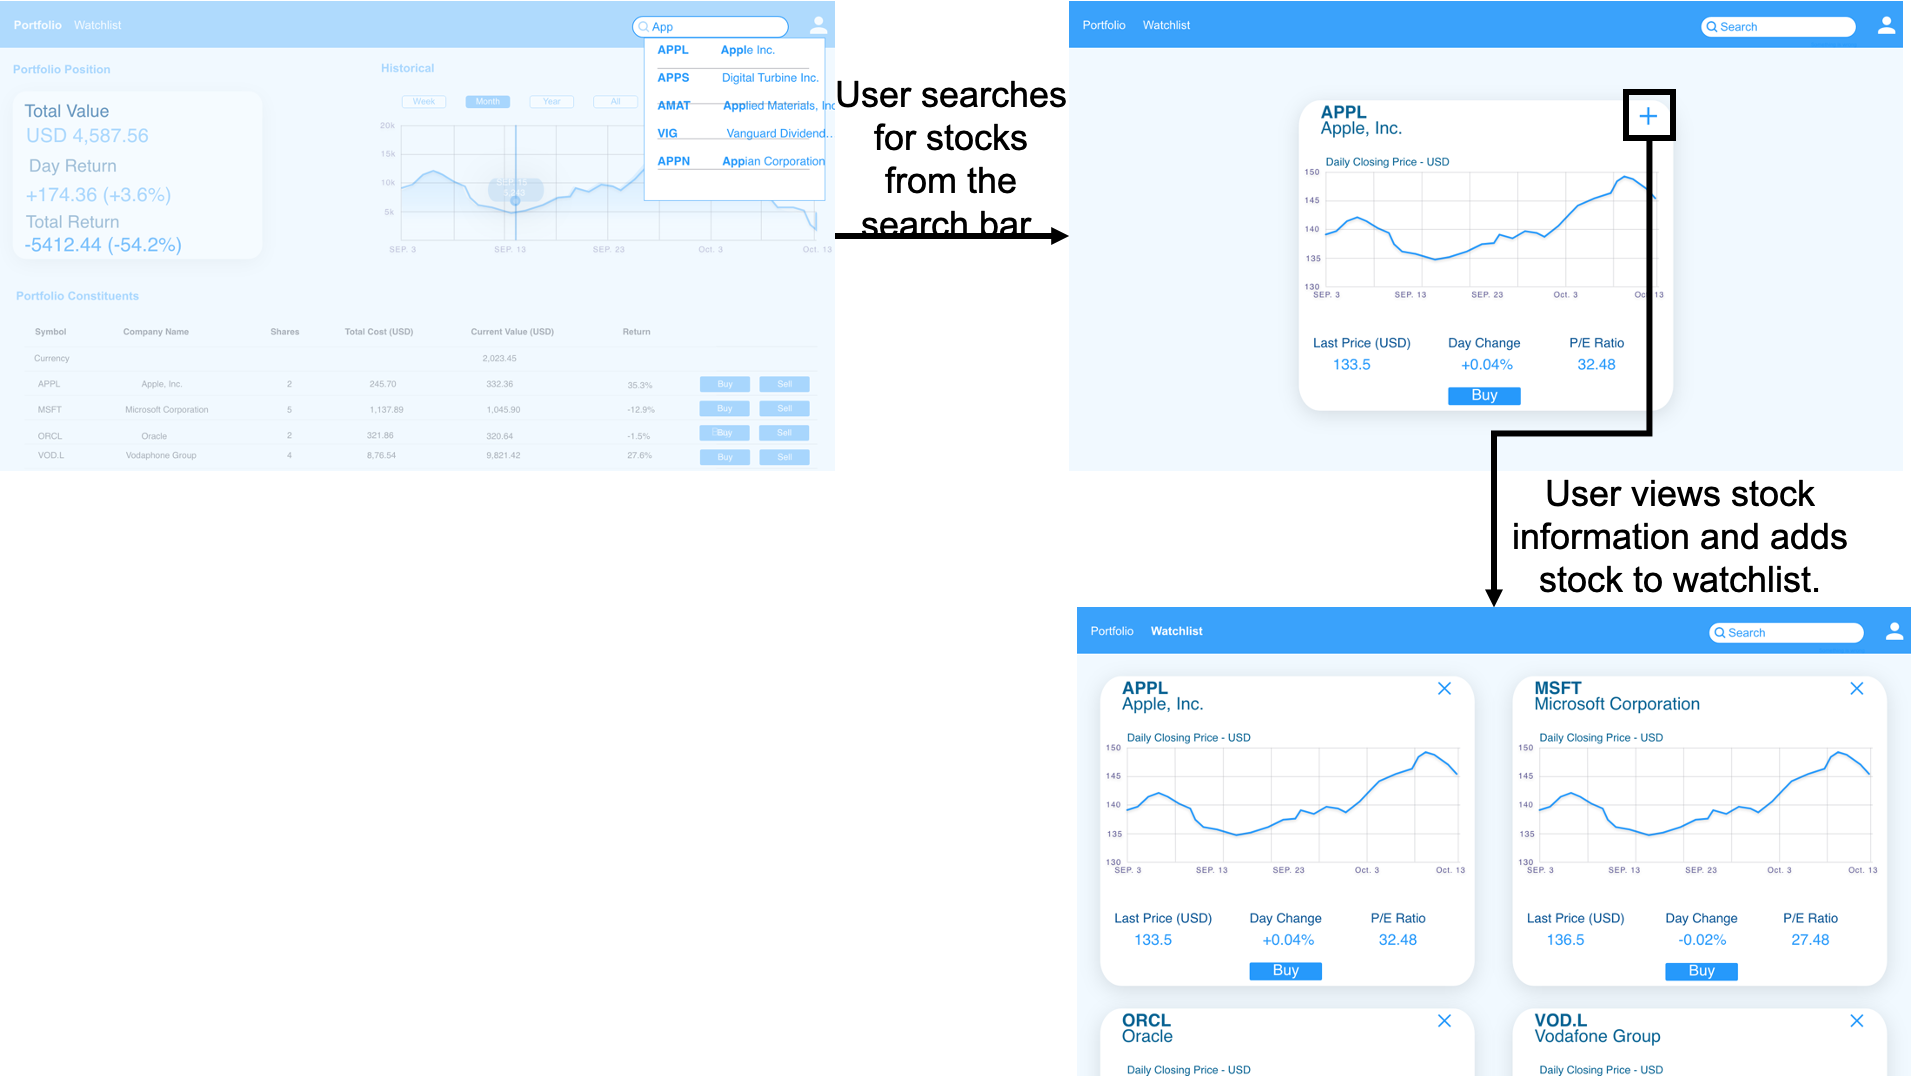
\includegraphics[scale = 0.5]{./3_story_boards/Search.png}
    \caption{Search wire-frame}
    \label{fig:search}
\end{figure}
\break


\subsection{Buy Order}
\begin{figure}[h]
    \centering
    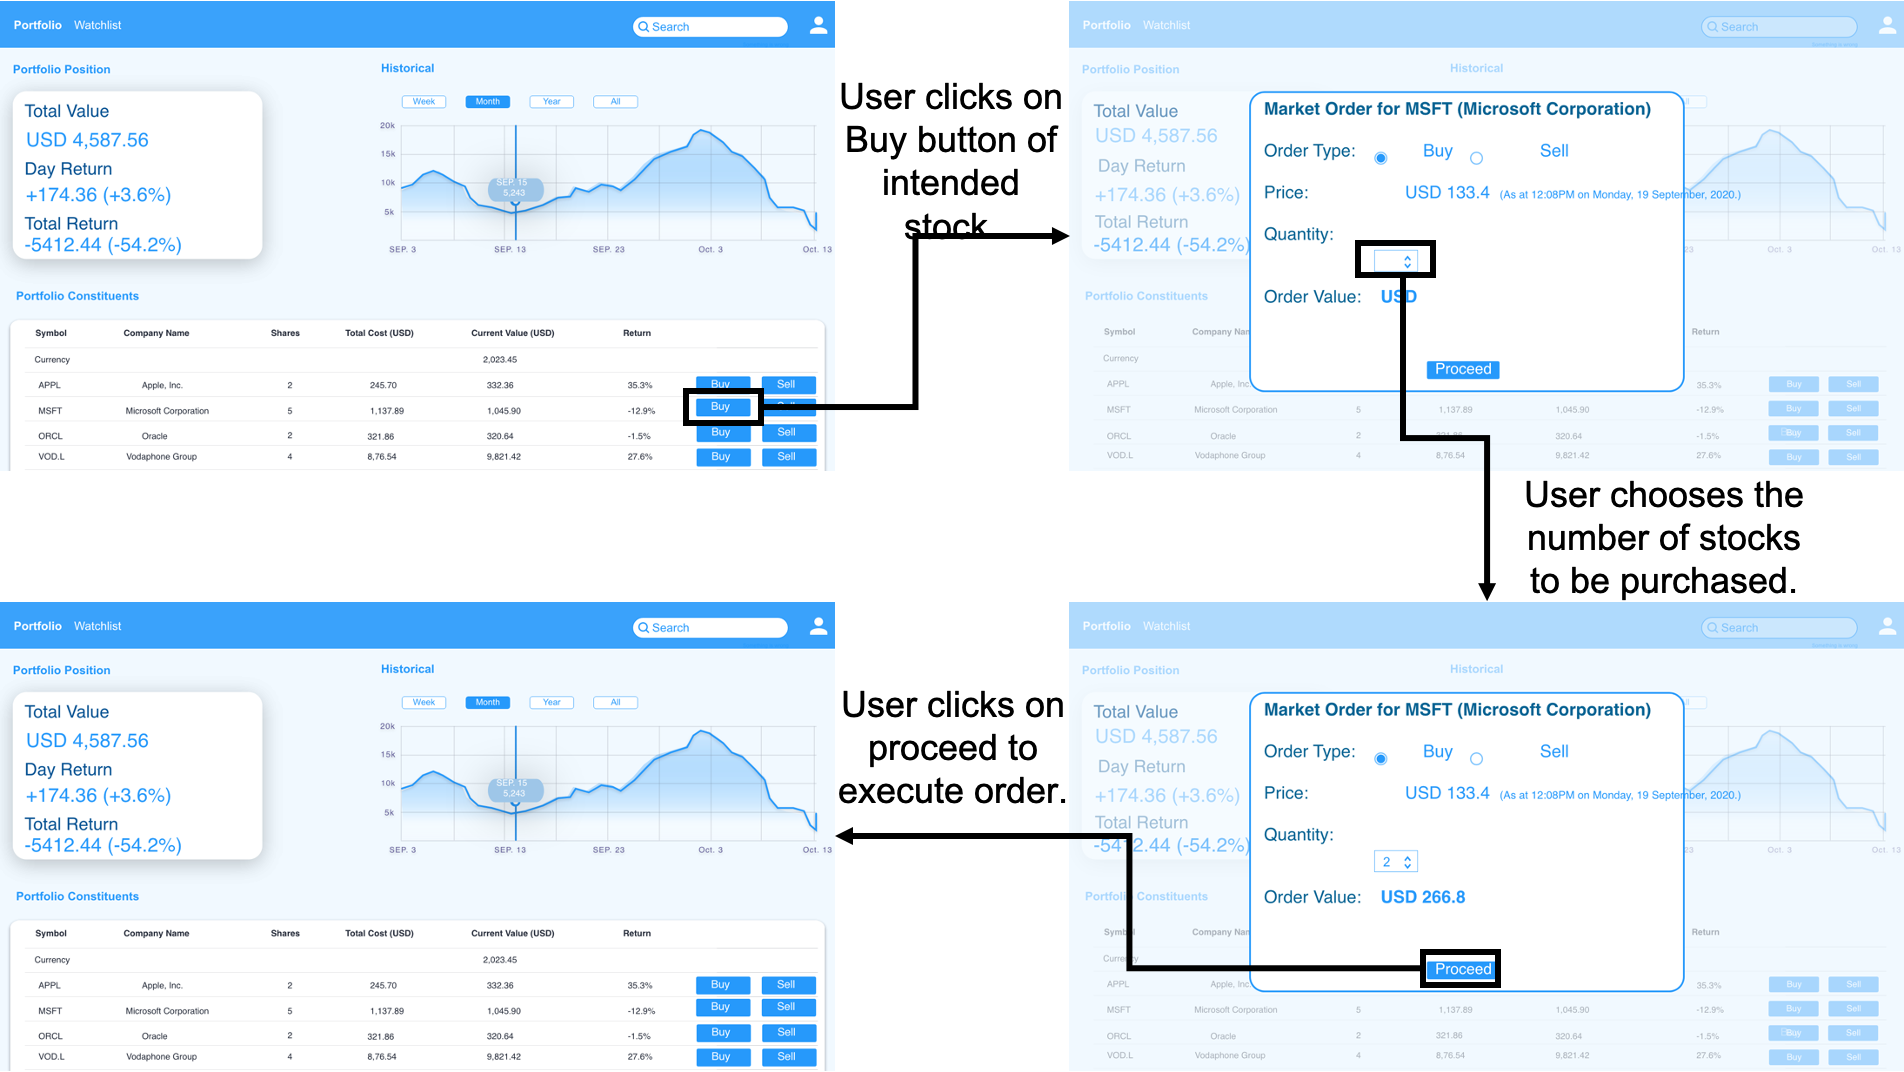
\includegraphics[scale = 0.5]{./3_story_boards/Buy.png}
    \caption{Buy wire-frame}
    \label{fig:buy}
\end{figure}
\break

\subsection{Sell Order}
\begin{figure}[h]
    \centering
    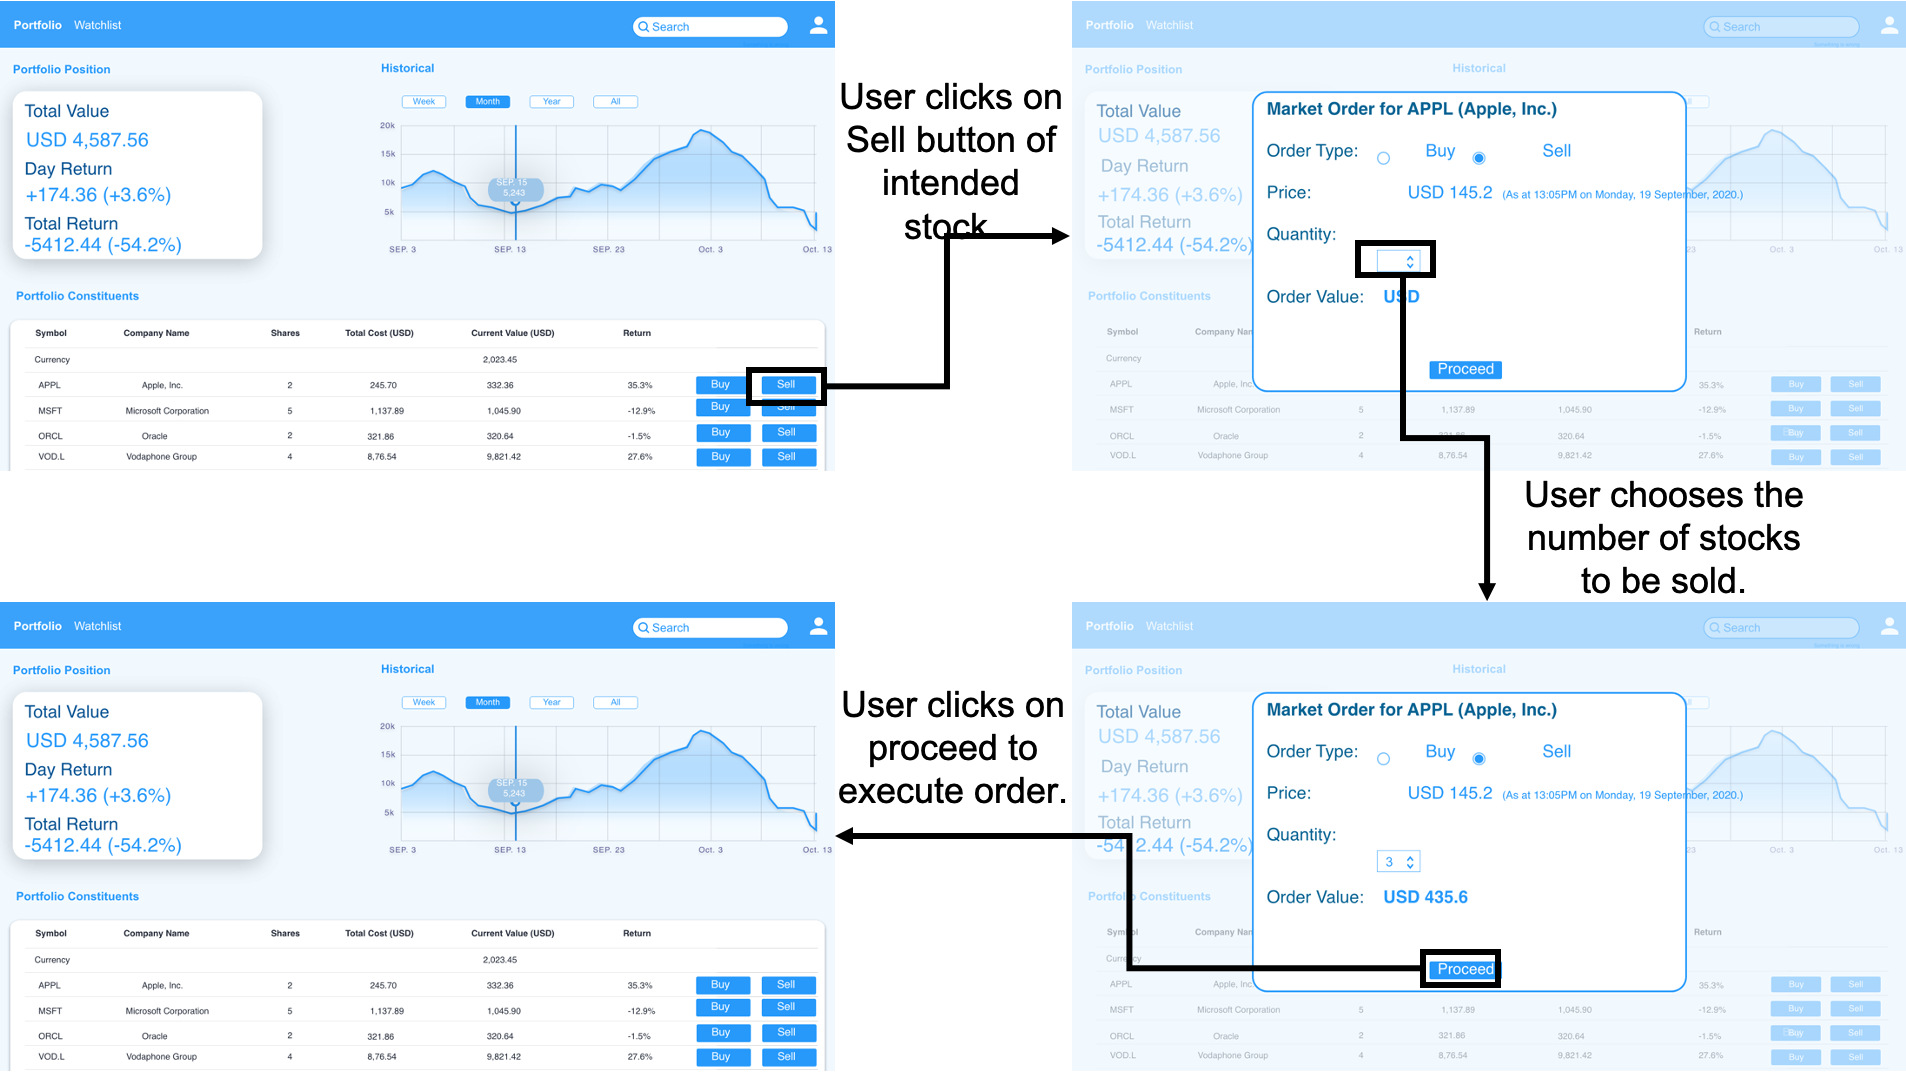
\includegraphics[scale = 0.5]{./3_story_boards/Sell.png}
    \caption{Sell wire-frame}
    \label{fig:sell}
\end{figure}
\break


\subsection{User Logout}
\begin{figure}[h]
    \centering
    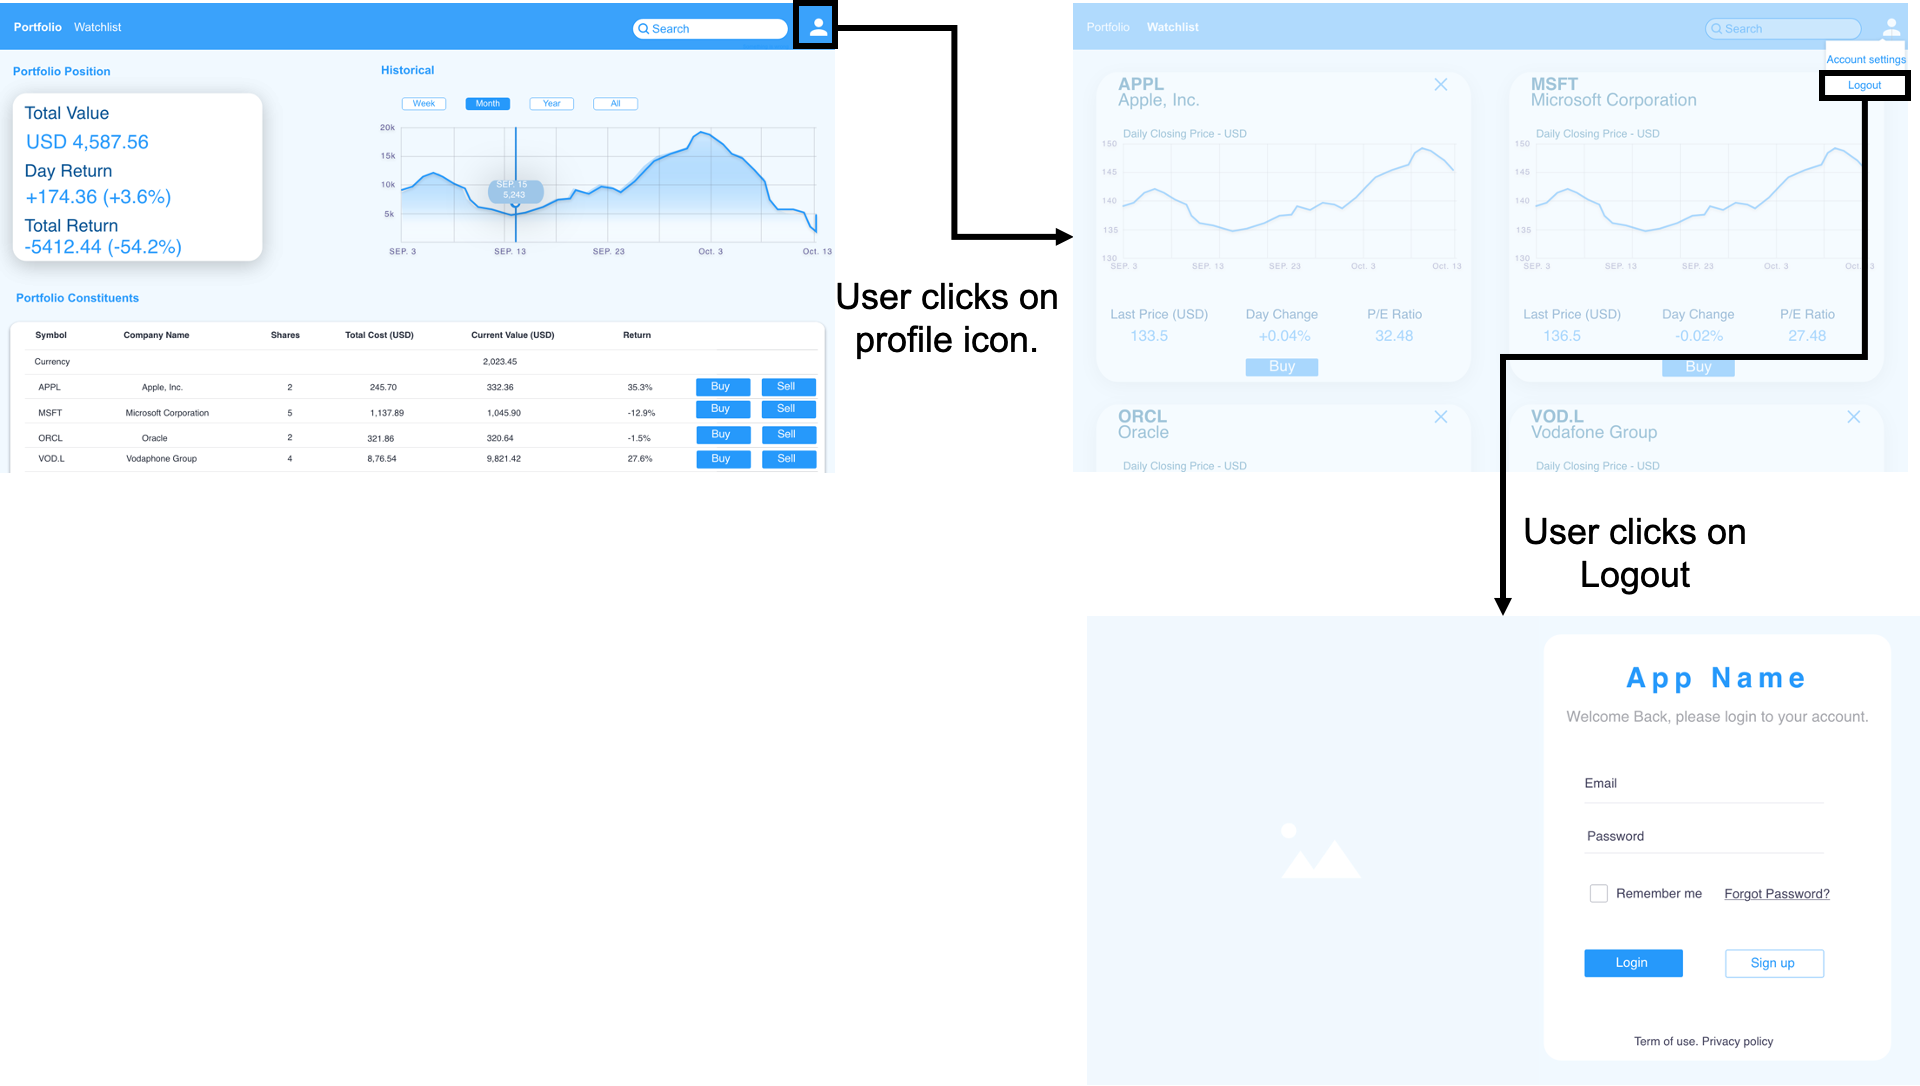
\includegraphics[scale = 0.5]{./3_story_boards/Logout.png}
    \caption{Logout wire-frame}
    \label{fig:logout}
\end{figure}
\break


\subsection{Password Reset}
\begin{figure}[h]
    \centering
    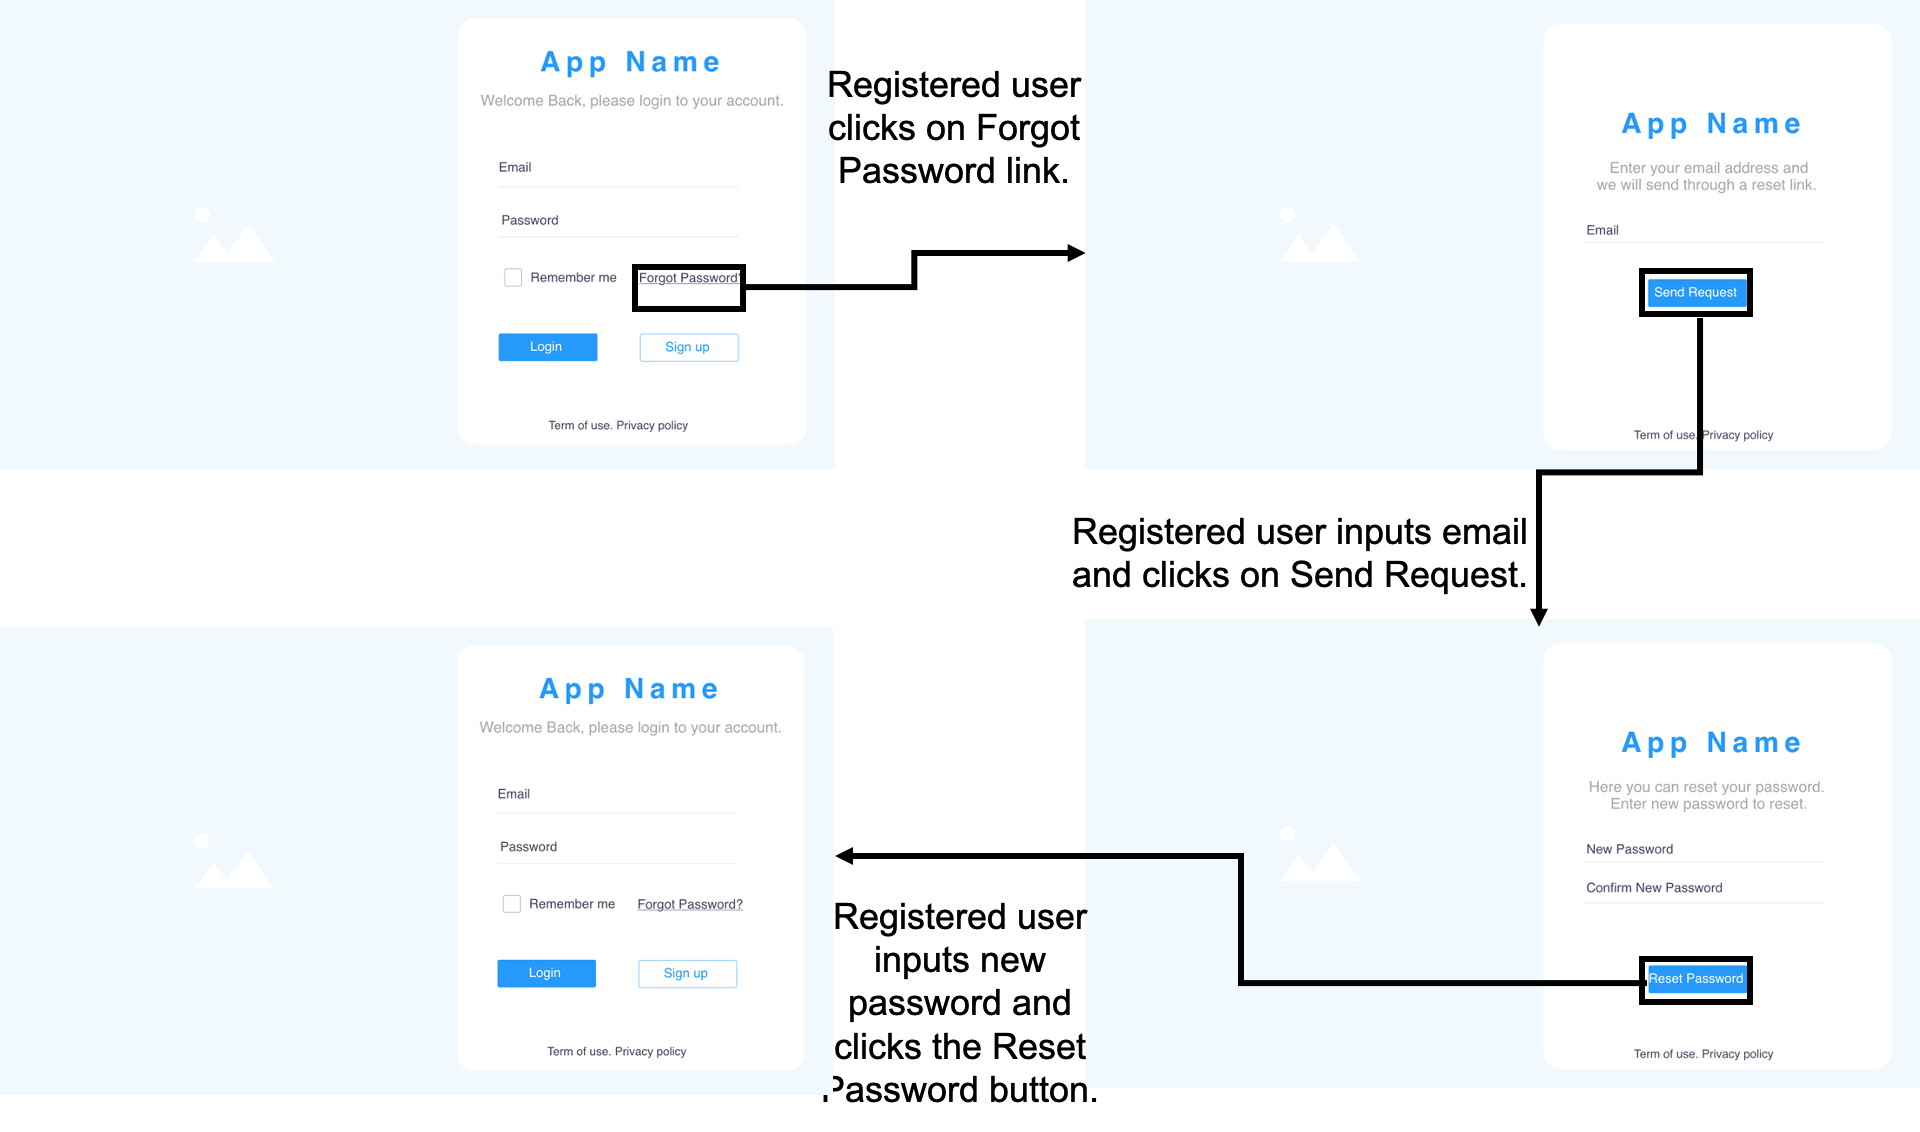
\includegraphics[scale = 0.5]{./3_story_boards/Password.png}
    \caption{Password reset wire-frame}
    \label{fig:password}
\end{figure}
    % !TEX root = ..\proposal.tex

\section{Architecture}
    \label{sec:arch}

{\color{red}
A CLEAR DESCRIPTION SHOWING THE PRESENTATION, BUSINESS AND DATA LAYERS IN THE
SYSTEM, AND WHAT EACH LAYER CONTAINS.\\

\noindent A CLEAR DESCRIPTION OF THE EXTERNAL ACTORS (EG: USER TYPES) AND HOW THEY INTERACT
WITH THE SYSTEM.\\

\noindent A CLEAR DESCRIPTION OF THE TECHNOLOGIES/LANGUAGES PLANNED FOR USE (EG: MYSQL,
SQL SERVER, MSMQ, .NET, JAVA, ETC), INCLUDING ALL THIRD PARTY FUNCTIONALITY PLANNED
TO BE USED (EG: CLOUDS/ SERVICES/ APIS/ LIBRARIES/ CODE).}



    \printbibliography
    
\end{document}
